O Bubble Sort é um algoritmo de ordenação simples onde a lista é percorrida da primeira até a última posição, comparando pares de elementos adjacentes e trocando-os se estiverem na ordem errada\cite{cormen2009introduction}. Este processo é repetido até que a lista esteja ordenada. Devido à sua natureza de comparação e troca, o Bubble Sort não é o método mais eficiente para listas grandes, mas sua implementação é direta e intuitiva. O algoritmo não
tem uma condição de parada, por isso as comparações são realizadas uma por uma mesmo array estando ordenado assim aumentando o seu tempo de execução.

\begin{figure}[h!]
    \centering
    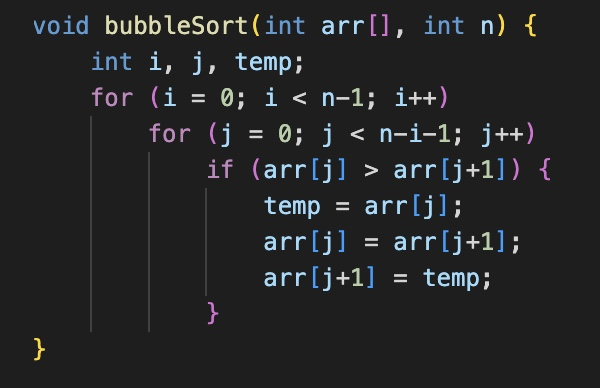
\includegraphics[width = 10cm]{Imagens/Bubble Sort/ImagemBubble.jpg}
    \caption{ALgoritmo Bubble Sort, imagem criada pelo autor.}
    \label{fig:imagembubble}
\end{figure}

Vamos entender o funcionamento do Bubble Sort com o seguinte exemplo \cite{sitebubble}: 
Entrada: arr[] = {6, 3, 0, 5}
Primeiro passo: O maior elemento é colocado em sua posição correta, ou seja, no final do array conforme na Figura \ref{fig:b1}.

\begin{figure}[h!]
    \centering
    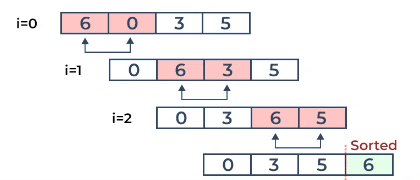
\includegraphics[width = 10cm]{Imagens/Bubble Sort/bubble1.png}
    \caption{Bubble Sort: colocando o maior elemento na posição correta.}
    \label{fig:b1}
\end{figure}

Segundo passo: Coloque o segundo maior elemento na posição correta, conforme na figura \ref{fig:b2}.

\begin{figure}[h!]
    \centering
    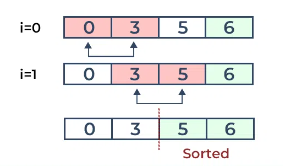
\includegraphics[width = 10cm]{Imagens/Bubble Sort/bubble2.png}
    \caption{Bubble Sort: colocando o segundo maior elemento na posição correta.}
    \label{fig:b2}
\end{figure}

Terceiro passo: Coloque os dois elementos restantes em suas devidas posições como mostra a figura \ref{fig:b3}.

\begin{figure}[h!]
    \centering
    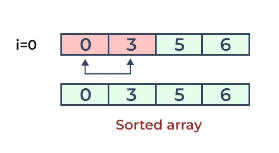
\includegraphics[width = 10cm]{Imagens/Bubble Sort/bubble3.png}
    \caption{Bubble Sort: colocando os elementos restantes em suas posições corretas.}
    \label{fig:b3}
\end{figure}